% !TEX root = dev-manual.tex
% ERA-Großpraktikum: Entwickleranleitung -- Allgemeines

\section{Allgemeines}
\label{dev:general}

Diese Sektion ist eine Einführung in die von uns genutzten Werkzeuge, welche für
die Entwicklung des Simulators benötigt werden. Das Ziel dieser Sektion ist es,
dass Leser am Ende in der Lage sind, eigenständig einen Build des Projekts
durchzuführen und somit am Projekt arbeiten können. Auch wird erläutert, welche
Beweggründe hinter der Auswahl an Werkzeugen stehen, von der wir uns erhoffen,
dass zukünftige Entwickler diese fortsetzen.

\subsection{Git}

Bei der Entwicklung von Software in einem Team ist es zwingend notwendig, viele
verschiedene Versionen derselben Software zu verwalten. Deshalb haben wir uns
für \emph{Git}\footnote{\url{https://git-scm.com/}} als Versionskontrollsystem
entschieden. Git erlaubt es uns, in isolierten \emph{Branches} parallel an
Features des Simulators zu arbeiten und im Falle eines Problems Veränderungen
auch rückgängig machen zu können. Ein weiterer Pluspunkt von Git ist die
komfortable Integration mit \emph{GitHub}, welches viele weitere Vorteile für
die verteilte Entwicklung eines großen Softwareprojekts, wie \erasim{}, bietet.

Da Git ein sehr mächtiges Werkzeug mit vielen möglichen Anwendungsweisen ist,
erfordert es zur effektiven Nutzung eine strukturierte Methodik. Diese Methodik
findet sich in der Industrie oftmals in Form von \emph{Git Flow}, welches
insbesondere ein Modell für die Verwendung von Branches vorschreibt.
\autoref{dev:git-flow} erläutert dieses Modell sowie das allgemeine Konzept von
Git Flow in mehr Detail.

\subsubsection{Git Flow}
\label{dev:git-flow}

\emph{Git
Flow}\footnote{\url{https://www.atlassian.com/git/tutorials/comparing-workflows/}}
ist ein beliebtes Modell der Git-Nutzung, welches vor allem bei der Verwaltung
von großen Projekten zum Einsatz kommt. Die von uns genutzte Variante lässt sich
wie folgt beschreiben:

\begin{itemize}
	\item Es gibt einen \emph{Master}-Branch, der immer die aktuellste, stabile Version enthält.
	\item Es gibt einen \emph{Development}-Branch, der den aktuellen Stand bei der Entwicklung
	einer neuen Version enthält. Der Code ist ebenfalls stabil, wenn auch manche Funktionen noch
	nicht vollständig sein können.
	\item Die einzelnen Aufgaben werden isoliert in einem \emph{Feature}-Branch bearbeitet.
	\item Ist eine Aufgabe fertig, so wird der entsprechende Feature Branch in den Development
	Branch gemerged.
	\item Ist eine neue Version auf dem Development Branch fertiggestellt, so wird die Development
	Branch in den Master Branch gemerged.
\end{itemize}

\subsubsection{Github}

Wir nutzen \emph{Github}\footnote{\url{https://github.com/}} als Hosting-Dienst
für den Simulator. Neben der einsteigerfreundlichen grafischen Oberfläche von
Github sind vor allem folgenden Funktionen hilfreich bei der Entwicklung:

\begin{itemize}
  \item \emph{Issues}: Die im vorherigen Kapitel genannten Aufgaben werden mit
  einem Issue verwaltet. Über die Nummer eines Issues lässt sich der Status der
  Entwicklung verfolgen.
  \item \emph{Pull Requests}: Nach der Fertigstellung eines Feature Branch wird
  ein Pull Request erstellt, sodass andere Entwickler den Code überprüfen und
  besprechen können.
	\item Integration von Tools wie
	\emph{Waffle}\footnote{\url{https://waffle.io/}} und \emph{Travis
	CI}\footnote{\url{https://travis-ci.org/}}
\end{itemize}

\subsection{C++}

Der Simulator ist zum Großteil in C++ geschrieben. Um von modernen Features und
Entwicklungen der C++ Sprache, beispielsweise Lambdas, Move-Semantik oder
Typinferenz mit \texttt{auto}, Gebrauch machen zu können, haben wir insbesondere
Wert darauf gelegt, die C++11 und C++14 Standards zu verwenden. Da diese
Features neuere Compiler benötigen, mussten wir eine untere Schranke für die
Versionen der von uns genutzten Compiler, \emph{gcc} und \emph{clang},
festlegen. Bei gcc (bzw. g++) liegt diese Schranke derzeit bei Version 5.0, bei
clang bei Version 3.7. Andere Compiler sind eventuell möglich, sofern sie C++14
unterstützen, wurden aber nicht getestet.

\subsubsection{Bibliotheken}

Die einzige, für das Endprodukt benötigte Abhängigkeit ist
\emph{Qt}\footnote{\url{https://www.qt.io/}} $\geq$ 5.6 in Kombination mit
QtQuick $\geq$ 2.6. Wir verwenden Qt zur Erstellung der grafischen Oberfläche,
haben aber grundsätzlich eine strikte Trennung zwischen Code der GUI und dem
Rest des Simulators. Durch diese Trennung wäre es möglich, den Simulator auch
ohne Qt zur Verfügung zu stellen, z.B. mit einer anderen Grafikbibliothek oder
als Kommandozeilenprogramm.  Eine Ausnahme zu dieser Trennung bildet die
Internationalisierung des Simulators. Der Simulator ist in der aktuellen Version
ausschließlich in Englisch verfügbar, uns war es aber ein großes Anliegen, auch
andere Sprachen unterstützen zu können. Somit verwenden wir die von Qt zur
Verfügung gestellten Mittel, für den Nutzer sichtbare Nachrichten übersetzbar zu machen,
auch in allen anderen Modulen außerhalb der GUI. So können z.B.
Prozessorarchitektur-spezifische Fehlermeldungen übersetzt werden.

\subsubsection{Code Style}

Da der Code nicht nur funktionieren, sondern auch gewissen Standards folgen
sollte, haben wir uns entschieden, den \emph{Google C++ Style Guide}
\footnote{\url{https://google.github.io/styleguide/cppguide.html}} als Grundlage
für unseren Code Style zu nutzen. Folgende Ausnahmen haben wir dabei festgelegt:

\begin{itemize}
  \item Präfix \texttt{\_}, anstatt Suffix \texttt{\_} für private Klassenattribute,
  \item \texttt{.hpp} und \texttt{.cpp} als Dateiendungen für C++
  Header und Implementierungen,
  \item Parameternamen werden im Header immer angegeben.
\end{itemize}

Um die Formatierung unseres Codes anhand dieser Regeln zu automatisieren
verwenden wir \texttt{clang-format}
\footnote{\url{http://clang.llvm.org/docs/ClangFormat.html}}. Dieses Werkzeug
entnimmt dem Programmier beispielsweise die Mühe, Parameternamen in langen
Funktionsaufrufen selbst einrücken zu müssen. Die Konfiguration von
\texttt{clang-format} liegt im YAML-Format in der Datei \texttt{.clang-format},
welche in der Wurzel des Projekts liegt.
\vspace{0.3cm}

\subsubsection{Dokumentation}

Neben diesem Bericht ist der gesamte Quellcode des Simulators in Form von
\emph{Doxygen}\footnote{\url{http://www.stack.nl/~dimitri/doxygen/}} Kommentaren
dokumentiert. Diese Dokumentation ist weitaus ausführlicher als dieser Bericht
und ist essentiell für die Weiterentwicklung des Simulators. Neben der
Möglichkeit, die Kommentare im Quellcode zu lesen, ist es mit Doxygen ebenfalls
möglich, eine HTML bzw. \LaTeX -Version der Dokumentation zu generieren. Dazu
wechselt man in das \texttt{docs/} Verzeichnis und führt den Befehl
\texttt{doxygen} aus, welcher anschließend die Dokumentation generiert.

\subsection{Build-Umgebung}
\label{sec:build-env}

Möchte man den Simulator selbst kompilieren, so wird eine \emph{Build-Umgebung}
vorausgesetzt. Da unser besonders Augenmerk auf Portabilität zwischen
Betriebssystemen liegt, wird in den folgenden Absätzen gezeigt, wie man eine
solche Umgebung unter den gängigen Betriebssystemen (Linux, macOS und Windows)
einrichten kann.

\subsubsection{Linux}

Da wir mit Qt 5.6 bzw. Qt 5.7 relativ neue Versionen von Qt verwenden, ist eine
reine Installation der Abhängigkeiten über die Paketverwaltung nur unter solchen
Linux Distributionen möglich, die auch die entsprechenden Versionen in den
Paketquellen beinhalten. Während dies unter Rolling Release Systemen (z.B. Arch
Linux) ein geringeres Problem ist, haben Anwender von Debian-basierten
Betriebssysteme häufiger mit älterer Software zu kämpfen. Unter Debian selbst
sind die benötigten Versionen erst ab Debian Stretch (Debian 9) verfügbar, unter
Ubuntu erst ab Version 16.10.

\begin{itemize}
	\item Debian basierte Betriebssysteme:
	\begin{lstlisting}
apt install build-essential cmake git qtdeclarative5-dev
	\end{lstlisting}

	\item Arch Linux:
	\begin{lstlisting}
pacman -S base-devel cmake git qt5-declarative \
  qt5-graphicaleffects qt5-quickcontrols
	\end{lstlisting}
\end{itemize}
\vspace{-0.2cm}
Ist eine Installation über die Paketquellen nicht möglich, bietet es sich an, Qt
manuell zu
installieren\footnote{\url{https://wiki.qt.io/Install_Qt_5_on_Ubuntu}}. Dafür
lädt man sich von der offiziellen Website einen Installer runter, der nach dem
Start einen Installationsort erfragt. Dieser muss später beim Bauen des Projekts
angegeben werden.
\vspace{0.4cm}

\pagebreak
\subsubsection{Aufsetzen von QtCreator}

QtCreator ist eine integrierte Entwicklungsumgebung, die von Qt selbst zur Verfügung gestellt wird und somit alle Features von Qt (qml, Widget-Designer, ...) nativ unterstützt. Da die IDE auch C++-Programmierung unterstützt, eignet sie sich als Alrounder-IDE für dieses Projekt.\\

Im Folgenden wird das Aufsetzen von QtCreator und erste Schritte danach für \textbf{Ubuntu 16.10} beschrieben:\\

\textbf{QtCreator installieren}\\
Über den Paketmanager:
\begin{lstlisting}
apt install qtcreator
\end{lstlisting}

\textbf{Repository klonen}\\
Siehe \autoref{dev-report-cmake-build}. Endet die Ausführung von cmake in einem Fehler (``Could not find a package configuration file provided by Qt5Widgets``), dann ist vermutlich bei der Installation von \texttt{qtdeclarative5-dev} etwas schiefgegangen.\\

\textbf{In QtCreator CMake-Projekt einrichten}\\
Im Startbildschirm ``Open Project`` und dann die oberste \texttt{CMakeLists.txt} (die in \texttt{era-gp-sim/CMakeLists.txt}) öffnen.\\
Im Reiter ''Configure Project'' für das Kit ''Desktop'' -> Details: Nur Debug und Release anhaken und die Build-Ordner anpassen\footnote{Es bietet sich an, für die IDE einen anderen Build-Ordner zu verwenden, als für das Bauen über die Konsole. Ein CMake-Projekt in QtCreator wird mit CodeBlocks erzeugt und erstellt daher leicht andere Konfigurationsdateien als cmake über die Konsole. Damit beides parallel nebeneinander betrieben werden kann, sollten die Build-Ordner getrennt werden.}. Die Auswahl bestätigen.\\
Jetzt sollte das Edit-Tab mit dem Projekt geöffnet sein. Im unteren Rand unter ''General Messages'' sollte einmal cmake automatisch aufgerufen worden sein, links oben im ''Projects'' Fenster sollte die Struktur des Projekts (mit CMakeLists.txt, include, source, tests und third-party) zu sehen sein.\\
Im Projects-Tab (linker Rand, Schraubenschlüssel) im Reiter ''Build \& Run'' wird jetzt der Build-Prozess konfiguriert.
Bei ''Edit build configuration'' Debug auswählen, dann unter ''Build Steps'' folgendes verändern:\\
\includegraphics[scale=0.5]{images/setup-qtcreator-build-config.png}\\
Der Eintrag von cmake Arguments soll dabei der relative Pfad vom eingetragenen Build-Ordner zum obersten Ordner des Projekts sein. Im Beispiel ist der Build-Order unter \texttt{era-gp-sim/build\_qtcreator\_debug} angelegt, d.h. eine Ebene höher liegt der root-Ordner des Projekts. Das \texttt{-j4} Argument bei \texttt{make} erhöht die Geschwindigkeit beim Bauen, da 4 Jobs gleichzeitig ausgeführt werden.
Zur Run-Konfiguration wechseln 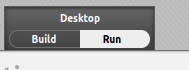
\includegraphics[scale=1.0]{images/setup-qtcreator-run-config.png} und als ''Working Directory'' den Build-Ordner eintragen.\\

Nun zurück wechseln und bei ''Edit build configuration'' Release auswählen und sowohl ''Build Steps'' als auch ''Run'' wie oben verändern.\\

Ins Edit-Tab wechseln und am linken Rand unten beim Monitor von ''Release'' auf ''Debug'' wechseln und dann mit Klick auf den Hammer das Projekt bauen.\\
\includegraphics[scale=0.7]{images/setup-qtcreator-change-build-flavor.png}\\
Hier können dann auch später statt ''era-sim'' verschiedene Test-Suits lokal ausgeführt werden. In der ''Compile Output'' Konsole kann der Fortschritt des Bauvorgangs überwacht werden.\\


\textbf{Nützliche Einstellungen}\\
\begin{itemize}
	\item File Naming:\\
	Im Menü \texttt{Tools -> Options}, dort in der linken Auswahlliste C++ -> Reiter ''File Naming'':\\
	Bei Headers Suffix zu hpp ändern.
	\item Lizenz automatisch einfügen:\\
	Im Menü \texttt{Tools -> Options -> C++ -> FileNaming}: Unter ''License Template'' kann der Pfad zu einer Textdatei eingegeben werden, deren Inhalt dann als Kommentar an den Anfang jeder neu erzeugten Datei platziert wird.
	\item Auto-Formatting (Plugin):\\
	 Muss evtl. über \texttt{Help -> About plugins} herunterladen (''Beautifier''). Ist dann unter \texttt{Tools -> Options -> Beautifier} zu finden.
\end{itemize}

\textbf{Erste Schritte}\\
\begin{itemize}
	\item Neue Datei erstellen:\\
	\texttt{File -> New File or Project}
	\item Aktuelle Datei formatieren:\\
	\texttt{Tools -> Beautifier -> ClangFormat -> Format Current File}
\end{itemize}


\pagebreak

\subsubsection{macOS}

Im Folgenden wird beschrieben, wie die Build-Umgebung für \erasim{} auf macOS
aufgesetzt werden kann.

\paragraph{Qt installieren}

Um Qt auf einem Mac-Computer zu installieren, bietet es sich an, den Installer
zu verwenden, den man über die offizielle Website herunterladen
kann\footnote{\url{https://www.qt.io/download/}}. Bei der Installation können
neben der aktuellsten auch ältere Versionen des \emph{Frameworks}
heruntergeladen werden. Nach der Installation befindet sich am angegebenen
Installationspfad ein Ordner \texttt{Qt}, in dem sich auch der QtCreator-IDE
befindet.

\paragraph{CMake aktualisieren}

Zum Bauen des Projekts wird CMake benötigt, das in der Regel über einen
Paketmanager installiert oder alternativ von der offiziellen Website
heruntergeladen werden kann.

\paragraph{In QtCreator ein CMake-Projekt erstellen}

Um ein CMake-Projekt in QtCreator einzurichten, können die gleichen Schritte, wie
im Kapitel für Linux beschrieben, durchgeführt werden.

\subsubsection{Windows}

Unter Windows ähnelt der Vorgang jenem auf macOS. Die Installation von Qt ist
mit einem Installer am angenehmsten, wobei es empfehlenswert ist, die Open
Source Version von Qt zu verwenden. Des Weiteren haben wir die besten
Erfahrungen mit MinGW\footnote{\url{http://www.mingw.org/}} gemacht, da der Qt
Installer anbietet, dies automatisch zu installieren. Schließlich wird noch
CMake benötigt, was man sich von der offiziellen Website herunterladen kann. Mit
QtCreator ist der Einrichtungsaufwand am geringsten, da etwaige Pfade zu
Bibliotheken automatisch gesetzt werden. Die Einrichtung entspricht den
gleichen Schritten, wie im Kapitel für Linux.

Unter Windows gibt es zugegebenermaßen die meisten Probleme, da viele kleine
Faktoren mitspielen. Bei Problemen sollte die Suchmaschine der Wahl, oder gleich
eine virtuelle Maschine mit einem Linux für die Entwicklung verwendet werden.

\pagebreak
\subsection{CMake und Make}
\label{sec:cmake-make}

Um auch den Build Prozess unabhängig vom Betriebssystem durchzuführen, haben wir
uns für \emph{CMake}\footnote{\url{https://cmake.org/}} entschieden. CMake kann
die benötigten \texttt{Makefiles} (wenn gewünscht auch \emph{Ninja}-Files oder
\emph{XCode}-Projekte) generieren, welche anschließend von
\emph{Make}\footnote{\url{https://www.gnu.org/software/make/}} ausgeführt werden
können.

Um einen Build des Projekts durchzuführen, sollte vorher eine entsprechende
Build-Umgebung aufgesetzt werden (siehe \autoref{sec:build-env}). Anschließend
kann mit den Folgenden Befehlen ein neuer Build erzeugt werden:

\begin{lstlisting}[language=bash, keywords={}]
# Projekt herunterladen
git clone https://github.com/TUM-LRR/era-gp-sim

# In das Projektverzeichnis wechseln
cd era-gp-sim

# Submodule initialisieren (Google Test)
git submodule update --init

# Build Verzeichnis erstellen und betreten
mkdir build && cd build

# Mit CMake die Makefiles erzeugen
cmake ..

# Projekt bauen (Die Option -j setzt Anzahl an
# Jobs und beschleunigt so den Build Prozess)
make -j 4

# Programm starten
./bin/era-sim
\end{lstlisting}

Hat man Qt manuell installiert, ist es ggf. notwendig, den Installationspfad bei der
Ausführung von CMake zu spezifizieren.

\begin{lstlisting}[language=bash, keywords={}]
# Wurde z.B. der Ordner ~/Qt5.7.0 bei der manuellen
# Installation von Qt angegeben, so muss man CMake mit
# dem folgenden Argument aufrufen:
cmake -D CMAKE_PREFIX_PATH=~/Qt5.7.0/5.7/gcc_64 ..
\end{lstlisting}

Alternativ ist es auch möglich, mit QtCreator zu arbeiten. Dabei öffnet man das
\texttt{CMakeLists.txt} als Projekt, und hat so eine grafische Oberfläche für
die Entwicklung am Simulator. Auch CMake/Make muss so nicht mehr manuell über
die Kommandozeile bedient werden, ein Build kann über die grafische Oberfläche
von QtCreator erzeugt werden (siehe \autoref{para:setup-qtcreator}).

\subsection{Tests}

Wir nutzen das
\emph{GoogleTest}\footnote{\url{https://github.com/google/googletest}} Framework
zur Automatisierung unserer Tests. Die Tests befinden sich im \texttt{tests/}
Verzeichnis, gruppiert nach ihren Modulen. Da Tests der grafischen Oberfläche zu
komplex wären, haben wir uns auf die übrigen Module des Simulators beschränkt,
deren korrekte Funktionalität in jeweils separaten \emph{Unit-Tests} überprüft
wird.

Um ein einheitliches Ergebnis bei den Tests zu erzielen, nutzen wir das
Continuous Integration Tool \emph{Travis
CI}\footnote{\url{https://travis-ci.org/}}. Dabei wird nach jedem hochgeladenen
Commit ein Clean Build angefertigt, der alle verfügbaren Tests durchführt. Das
Ergebnis dieses Tests wird auf Github veröffentlicht und ist bindend. Die Tests
werden sowohl mit gcc, als auch mit clang durchgeführt. Die Konfiguration von
Travis befindet sich in der Datei \texttt{.travis.yml}

Die Tests können auch lokal ausgeführt werden. Dazu wechselt man in das Build
Verzeichnis und nutzt das mit CMake mitgelieferte Programm \texttt{ctest} um die
Tests zu starten. Um die Testgeschwindigkeit zu erhöhen empfiehlt es sich, mit
der \texttt{-j} Option die Anzahl der Jobs zu erhöhen (beispielsweise
\texttt{-j4} auf einem Quad-Core Rechner).

\subsection{Projektstruktur}

Mit der Größe des \erasim{}-Projekts wuchs mit der Zeit auch die Komplexität
unserer Ordnerstruktur. So befinden sich nun in unserem Repository viele
verschiedene Ordner, die Code, Konfigurationsdateien des Simulators, Tests,
Hilfs-Skripte oder Beispielprogramme enthalten. Genauer arbeiten wir momentan
mit folgenden Verzeichnissen:

\begin{itemize}
	\item \textbf{\texttt{docs/}} enthält die Dokumentation von \erasim{}, also
	die Berichte und die Konfiguration von Doxygen.
	\item \textbf{\texttt{examples/}} enthält Beispielprogramme für RISC-V.
	\item \textbf{\texttt{include/}} enthält alle C++ Header Dateien, gruppiert
	nach ihrem Modul. Wir haben uns um die strikte Trennung zwischen Header- und
	Source Dateien bemüht.
	\item \textbf{\texttt{installer/}} enthält die Konfigurationsdateien für
	den Installer von \erasim{}.
	\item \textbf{\texttt{isa/}} enthält die Architekturdefinitionen in YAML und
	JSON Konfigurationsdateien.
	\item \textbf{\texttt{scripts/}} enthält für die Entwicklung nützliche
	Skripte, um z.B. neue Klassen zu erstellen (inklusive Header- und
	Source Datei).
	\item \textbf{\texttt{source/}} enthält C++ Source Dateien, ebenfalls
	gruppiert nach ihren Modulen. Auch hier sei auf die strikte Trennung
	zwischen Header- und Source Dateien verwiesen.
	\item \textbf{\texttt{tests/}} enthält die Unit Tests jeder Module.
	\item \textbf{\texttt{third-party/}} enthält genutzte Bibliotheken. Konkret
	wird Google Tests dadurch eingebunden und ein JSON Parser bereitgestellt.
\end{itemize}

\subsection{Release}

Wegen Abhängigkeiten zu Qt bzw. QtQuick und Konfigurationsdateien, wie
\texttt{isa-} und \texttt{themes-}Ordner fallen bei jedem Betriebssystem noch
Dateien neben der ausführbaren Programmdatei an. Eine Auslieferung soll trotzdem
für den Endnutzer möglichst einfach sein, daher haben wir uns für eine
Installation per Installer entschieden.

Das Qt Installer
Framework\footnote{\url{https://wiki.qt.io/Qt-Installer-Framework}} bringt
hierbei eine Lösung mit einigen Vorteilen mit. Das Verhalten bzw. die
Konfiguration des Installer wird über JavaScript und XML ermöglicht, so ist
keine Kompilierung nötig. Außerdem bietet das Framework eine Abstraktion des
Ziel-Betriebssystems, so lassen sich mit einer Konfiguration die Installer für
alle drei unterstützte Plattformen erzeugen. Der Installer liefert dabei
lediglich die Nutzlast (eine gepackte Version des Simulators) an den vom
Benutzer benannten Speicherort und erzeugt Verknüpfungen.

\subsubsection{Konfiguration des Installers}
\begin{figure}[H]
	\begin{center}
		\begin{tikzpicture}[%
      thick,
		grow via three points={one child at (0.8,-0.8) and
			two children at (0.8,-0.8) and (0.8,-1.7)},
		edge from parent path={($(\tikzparentnode\tikzparentanchor)+(.2cm,0pt)$) |- (\tikzchildnode\tikzchildanchor)},
		growth parent anchor=west,
		parent anchor=south west]

		\tikzstyle{every node}=[%
      draw=black,
      anchor=west,
      rounded corners=1pt,
      font=\ttfamily
    ]

		\node {\erasim}
		child { node {installer/}
			child { node {config/}
				child {node {config.xml} }
			}
			child [missing]{}
			child { node {packages/}
				child {node {erasim.base/}
					child {node {meta/}
						child {node{ package.xml} }
					}
					child [missing]{}
					child {node {data/}
						child {node {archive.7z}
						}
					}
					child [missing]{}
				}
				child [missing]{}
				child [missing]{}
				child [missing]{}
				child [missing]{}
				child {node {erasim.shortcut/}
					child { node {...} }
				}
			}
		};
		\end{tikzpicture}
	\end{center}
	\caption{Struktur der Installerkonfiguration}
	\label{dev-manual-installer}
  \vspace{-0.4cm}
\end{figure}

Die Konfiguration des Installer (z.B. Aussehen, voreingestellte Pfade) wird in
der Datei \texttt{config.xml} im Ordner \texttt{config} vorgenommen. Die
auszuliefernden Dateien sind dabei in Pakete unterteilt. Die Installation dieser
Pakete kann der Nutzer an- und abwählen. \texttt{erasim.base} enthält die
Installation des Simulators. Diese wird an den vom Nutzer angegebenen Ort
(standardmäßig unter Windows z.B \texttt{C:$\backslash$Programme} unter Linux
\texttt{/opt/}) entpackt. \texttt{erasim.shortcut} liefert keine Dateien aus,
sondern erstellt einen Startmenüeintrag unter Windows bzw. einen Desktopeintrag
unter Unix.

\subsubsection{Erzeugen des Installers}

Das Framework besteht aus mehreren Tools, die zum Erzeugen notwendig sind.
\texttt{archivegen} verpackt angegebene Daten in ein .7z Archiv.
\texttt{binarycreator} erzeugt den Installer aus den Archivdaten und der
Konfiguration. Die genauen Schritte bis zum fertigen Installer variieren je nach
Betriebssystem, die Grundvorgehensweise ist jedoch gleich. Genaue Instruktionen
für jedes Betriebssystem sind im \texttt{README} des \texttt{installer} Ordners
zu finden. Die Grundschritte sind
\begin{itemize}
	\item Saubere Version mit Optimierung und ohne Debug-Symbole bauen;

	\item Executable und alle benötigten Qt- und Compiler-Bibliotheken sowie alle
	verwendeten QtQuick/QML Module zusammen mit \texttt{isa} und
	\texttt{themes}-Ordner mit \texttt{archivegen} in ein Archiv zusammenfügen.
	Dieses Archiv kommt nach \texttt{installer/packages/erasim.base/data/};

	\item Das Programm \texttt{binarycreator} ausführen, um den Installer zu
	bauen.

\end{itemize}
